\documentclass[a4paper, 16pt]{article}
\usepackage[utf8]{inputenc}
\usepackage[english, russian]{babel} 
\usepackage[left=20mm, top=20mm, right=20mm,
 bottom=20mm, head=1mm, foot=1mm]{geometry}
\usepackage{tikz} 
\usepackage{amsmath, amsfonts, amssymb}
\usepackage{graphicx}
\usepackage{fancybox, fancyhdr}
\usepackage{hyperref}
\usepackage{listings}
\usepackage{caption}
\usepackage{subcaption}
\usepackage{xcolor}
\pagestyle{fancy}
\fancyhf{}
\fancyhead[L]{Лабораторная работа №2}
\fancyhead[R]{Частотные методы}
\fancyfoot[C]{\thepage}
\graphicspath{{images/}}
\usetikzlibrary{patterns}
\definecolor{LightGray}{gray}{0.95}
\lstdefinestyle{pycode}{
    language=Python,
    basicstyle=\footnotesize\ttfamily,
    numbers=left,
    numberstyle=\tiny\color{gray},
    stepnumber=1,
    numbersep=5pt,
    backgroundcolor=\color{LightGray},
    showspaces=false,
    showstringspaces=false,
    showtabs=false,
    tabsize=4,
    captionpos=b,
    breaklines=true,
    breakatwhitespace=false,
    frame=single,
    rulecolor=\color{black},
    linewidth=\linewidth,
    keywordstyle=\color{red}\bfseries,
    commentstyle=\color{green!40!black},
    stringstyle=\color{purple},
    escapeinside={\%*}{*)},
    xleftmargin=0pt,
    framexleftmargin=0pt,
    framexrightmargin=0pt
}
\lstset{style=pycode}
\hypersetup{
    colorlinks=true,
    linkcolor=blue,
    filecolor=magenta,      
    urlcolor=cyan,
    pdftitle={contents setup},
    pdfpagemode=FullScreen,
}
\allowdisplaybreaks
\newcommand{\frc}[2]{\raisebox{2pt}{$#1$}\big/\raisebox{-3pt}{$#2$}}

\begin{document}
\begin{titlepage}

    \begin{center}
    \vfill
    
    Федеральное государственное автономное образовательное учреждение высшего образования\\
    «Национальный Исследовательский Университет ИТМО»\ \\
    
    \vfill
    {\large\bf ЛАБОРАТОРНАЯ РАБОТА №2\\
        ПО ПРЕДМЕТУ «ЧАСТОТНЫЕ МЕТОДЫ»\\
        ПО ТЕМЕ «ПРЕОБРАЗОВАНИЕ ФУРЬЕ»}
    \vfill
        
    \begin{flushright}
        \begin{minipage}{.45\textwidth}
        {
            \hbox{Лектор: Перегудин А. А.}
            \hbox{Практик: Пашенко А. В.}
            \hbox{Студент: Румянцев А. А.}
            \hbox{Поток: ЧАСТ.МЕТ. 1.3}
            \hbox{}
            \hbox{Факультет: СУиР}
            \hbox{Группа: R3241}
        }
        \end{minipage}
    \end{flushright}
    
    \vfill
            
    Санкт-Петербург\\
    2024
    \end{center}
    \end{titlepage}
    \setlength{\parskip}{1.5mm}
    
    \tableofcontents

    \newpage
    \section{Введение}
    \noindent В заданиях 1 и 2 используется унитарное преобразование Фурье к угловой частоте $\omega$.\
    Подсчет Фурье- -образа производится по формуле ниже
    $$
    \hat{f}\left(\omega\right)=\dfrac{1}{\sqrt{2\pi}}\int\limits_{-\infty}^{\infty}f(t)e^{-i\omega t}\,dt
    $$
    

    \noindent В задании 3 используется преобразование Фурье к обыкновенной частоте $\nu$. В общем\
    виде формула имеет вид
    $$
    \hat{f}\left(\nu\right)=\int\limits_{-\infty}^{\infty}f\left(t\right)e^{-2\pi i \nu t}\,dt
    $$


    \noindent Для проверки равенства Парсеваля используется формула ниже
    $$
    \left|\left|f\right|\right|_2=||\hat{f}||_2,
    $$
    \noindent где $||f||_2$ -- вторая норма заданной фукнции, $||\hat{f}||_2$ -- вторая норма
    Фурье-образа функции $f$. Для нахождения нормы используются формулы, представленные ниже
    $$
    ||f(t)||_2=\sqrt{\int\limits_{a}^{b}f(t)\cdot f^{*}(t)\,dt},\,\,\,\,\,\,\,\,||\hat{f}(\omega)||_2=\sqrt{\int\limits_{a}^{b}\hat{f}(\omega)\cdot \hat{f}^{*}(\omega)\,d\omega}
    $$


    \noindent Все графики строятся программой, написанной на языке программирования python. В 1 и 2 заданиях\
    используется библиотека sympy, в задании 3 numpy и matplotlib. По ходу отчета приводится код для каждого задания.
    Для всех интегралов и графиков есть место с общими переменными и значениями -- файл static.py. Основные используемые
    данные приведены ниже
    \begin{lstlisting}[label=static, caption=Основные данные из файла static.py]
    from sympy import Symbol, Piecewise, Abs, sinc, E, oo

    t = Symbol('t')
    omega = Symbol('omega')

    interval = [-oo, oo]

    a_b_pars = [(1, 2), (2, 3), (3, 4)]
    consts = [-1, 0.5, 1]
    colors_strs = ['red', 'purple', 'blue', 'cyan'] 
    \end{lstlisting}


    \noindent В этом файле программно заданы функции, графики которых приводятся по ходу отчета. Также они необходимы
    для нахождения их Фурье-образа
    \begin{lstlisting}[label=funcs, caption=Программно заданные функции для заданий 1 и 2]
    def rectangular_function(a, b):
        return Piecewise((a, Abs(t) <= b), (0, Abs(t) > b))

    def triangular_function(a, b):
        return Piecewise((a - Abs(a * t / b), Abs(t) <= b), (0, Abs(t) > b))

    def cardinal_sinus(a, b):
        return a * sinc(b * t)
    
    def gaussian_function(a, b):
        return a * E ** (-b * t ** 2)
    
    def double_attenuation(a, b):
        return a * E ** (-b * Abs(t))
    \end{lstlisting}


    \section{Задание 1. Вещественное}
    \subsection{Прямоугольная функция}
    \noindent Рассмотрим прямоугольную функцию следующего вида
    $$
    f(t)=
    \begin{cases}
        a, & \left|t\right|\leq b,\\
        0, & \left|t\right|>b.
    \end{cases}
    $$


    % аналитическое выражение с выводом


    \noindent Рассмотрим программу. Сначала задается функция, принимающая параметры $a\text{ и }b$, после чего методом build\_{f}\_{t} строится график $f(t)$.
    На строке 10 приведен пример использования кода
    \begin{lstlisting}[label=f_t_rect, caption=Программа для построения графика прямоугольной функции]
    def build_f_t(f_t, clr, lbl):
        if (lbl == None):
            plot(f_t, line_color=clr, xlabel=r'$t$', ylabel=r'$f(t)$')
        else:
            plot(f_t, line_color=clr, xlabel=r'$t$', ylabel=r'$f(t)$', label=lbl, legend=True)

    build_f_t(rectangular_function(1, 2), 'red', None)
    \end{lstlisting}


    \noindent Построенные графики $f(t)$ для нескольких значений параметров $a,b>0$ расположены ниже
    \begin{figure}[htbp]
        \centering
        \begin{subfigure}{0.3\textwidth}
            \centering
            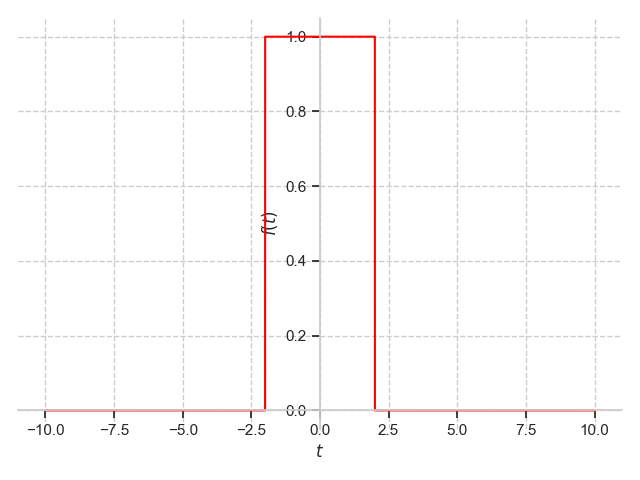
\includegraphics[width=\linewidth]{rectf_a=1_b=2.png}
            \caption{$a=1,\,\,b=2$}
            \label{fig:rectf_1}
        \end{subfigure}
        \hfill
        \begin{subfigure}{0.3\textwidth}
            \centering
            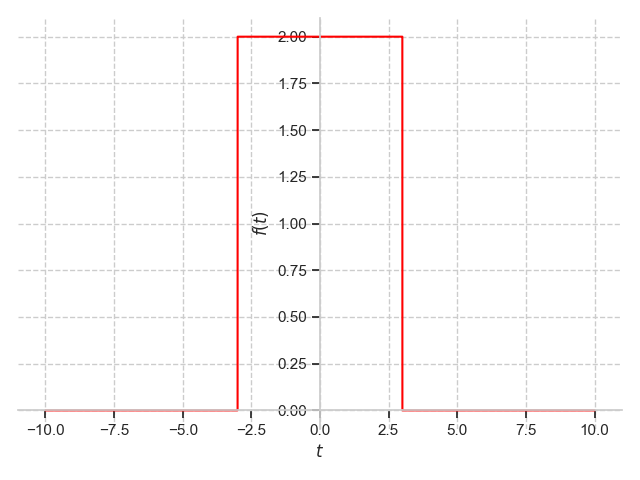
\includegraphics[width=\linewidth]{rectf_a=2_b=3.png}
            \caption{$a=2,\,\,b=3$}
            \label{fig:rectf_2}
        \end{subfigure}
        \hfill
        \begin{subfigure}{0.3\textwidth}
            \centering
            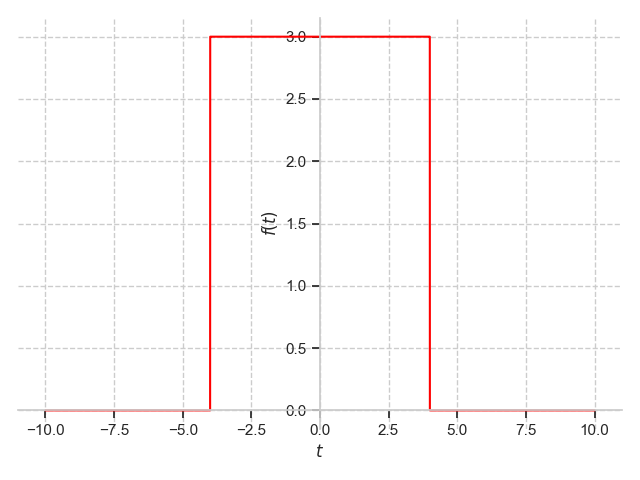
\includegraphics[width=\linewidth]{rectf_a=3_b=4.png}
            \caption{$a=3,\,\,b=4$}
            \label{fig:rectf_3}
        \end{subfigure}
        \caption{Прямоугольные функции при различных значениях $a$ и $b$}
        \label{fig:rectfs}
    \end{figure}


    \noindent Рассмотрим программу. Методом find\_{fimg} находится Фурье-образ заданной функции. Далее методом build\_{fimg2}
    строится график Фурье-образа. На 16-17 строчках находится пример использования кода
    \begin{lstlisting}[label=fimg_rect, caption=Программа для построения графика Фурье-образа некоторой функции $f(t)$]
    def find_fimg(f_t, lim1, lim2):
        integrand = f_t * E ** (-I * omega * t)

        result = integrate(integrand, (t, lim1, lim2))
        return coeff * result

    def build_fimg2(fimg, clr, lbl):
        if (lbl == None):
            plot(fimg, line_color=clr,
                 xlabel=r'$\omega$', ylabel=r'$c(\omega)$')
        else:
            plot(fimg, line_color=clr,
                 xlabel=r'$\omega$', ylabel=r'$c(\omega)$',
                 label=lbl, legend=True)
    
    rectfimg = find_fimg(rectangular_function, -oo, oo)
    build_fimg2(rectfimg, 'purple', None)
    \end{lstlisting}


    \noindent Построенные графики $\hat{f}\left(\omega\right)$ для тех же значений $a$ и $b$ расположены ниже
    \begin{figure}[htbp]
        \centering
        \begin{subfigure}{0.3\textwidth}
            \centering
            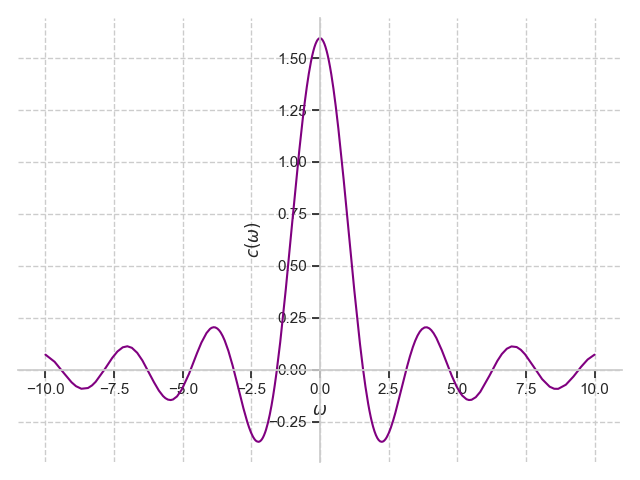
\includegraphics[width=\linewidth]{rectfimg_a=1_b=2.png}
            \caption{$a=1,\,\,b=2$}
            \label{fig:rectfimg_1}
        \end{subfigure}
        \hfill
        \begin{subfigure}{0.3\textwidth}
            \centering
            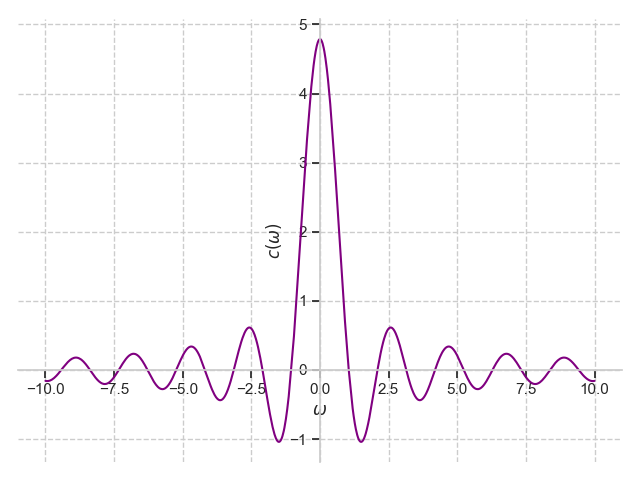
\includegraphics[width=\linewidth]{rectfimg_a=2_b=3.png}
            \caption{$a=2,\,\,b=3$}
            \label{fig:rectfimg_2}
        \end{subfigure}
        \hfill
        \begin{subfigure}{0.3\textwidth}
            \centering
            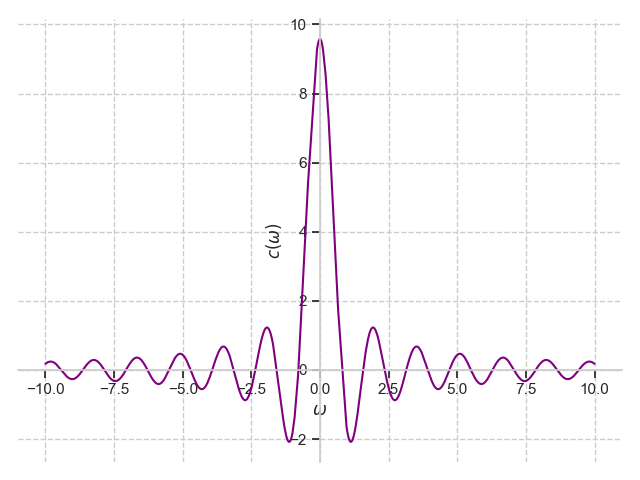
\includegraphics[width=\linewidth]{rectfimg_a=3_b=4.png}
            \caption{$a=3,\,\,b=4$}
            \label{fig:rectfimg_3}
        \end{subfigure}
        \caption{Фурье-образы прямоугольных функций при различных значениях $a$ и $b$}
        \label{fig:rectfimgs}
    \end{figure}


    % анализ графиков и ответы на вопросы


    \noindent Рассмотрим программу. Методом find\_{norm2} находится вторая норма переданной функции.
    Метод \\find\_{parseval} считает левую и правую части равенства Парсеваля. Пример использования кода
    расположен на 13-14 строчках листинга ниже
    \begin{lstlisting}[label=pars_rectf, caption=Программа для нахождения левой и правой сторон равенства Парсеваля]
    def find_norm2(f, lim1, lim2, var):
        integrand = f * conjugate(f)

        result = integrate(integrand, (var, lim1, lim2)).evalf()
        return sqrt(result).evalf()

    def find_parseval(f, fimg, lim1, lim2):
        pleft = find_norm2(f, lim1, lim2, t)
        pright = find_norm2(fimg, lim1, lim2, omega)

        return pleft, pright

    pl, pr = find_parseval(rectangular_function, rectfimg, -oo, oo)
    print(f'p_{1}: {pl} ?= {pr}')
    \end{lstlisting}


    \noindent Программа вывела в консоль результаты, представленные ниже
    \begin{lstlisting}[label=pres_rectf, caption=Результат выполнения программы для вычисления равенства Парсеваля]
    p_1: 2.00000000000000 ?= 2.0 + 0.e-114*I  
    p_2: 4.89897948556636 ?= 4.89897948556636 + 0.e-114*I 
    p_3: 8.48528137423857 ?= 8.48528137423857 + 0.e-114*I
    \end{lstlisting}


    \noindent Мнимыми частями в правой части равенства Парсеваля пренебрежем вследствие их стремления к нулю. В таком случае равенство Парсеваля выполняется, что можно объяснить тем, что интеграл позволяет
    рассмотреть норму непрерывно на заданном промежутке, а ряд только дискретно, вследствие чего теряются какие-то члены ряда,
    которых не хватает для выполнения равенства Парсеваля


    \subsection{Рассмотрим треугольную функцию следующего вида}
    $$
    f(t)=
    \begin{cases}
        a-\left|\dfrac{at}{b}\right|, & \left|t\right|\leq b,\\
        0, & \left|t\right|>b.
    \end{cases}
    $$


    % аналитическое выражение с выводом


    \noindent Для построения графиков треугольной функции сначала задается необходимая функция,
    после используется код, приведенный в пункте 2.1 для прямоугольной функции
    \begin{lstlisting}[label=triangf, caption=Программно заданная треугольная функция]
    null
    \end{lstlisting}


    \noindent Построенные графики $f(t)$ для нескольких значений параметров $a,b>0$ расположены ниже
    \begin{figure}[htbp]
        \centering
        \begin{subfigure}{0.3\textwidth}
            \centering
            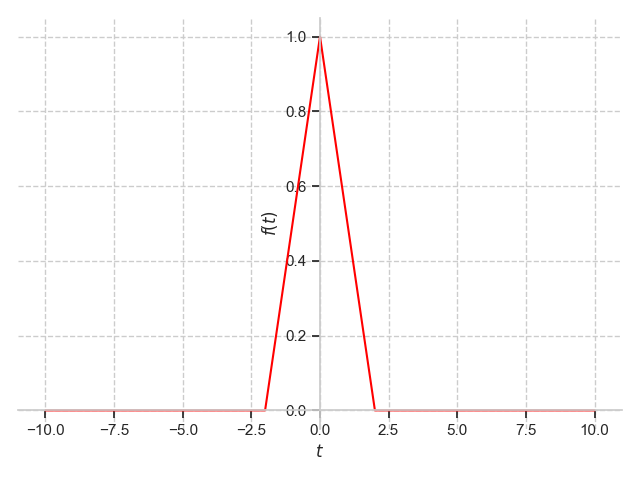
\includegraphics[width=\linewidth]{trif_a=1_b=2.png}
            \caption{$a=1,\,\,b=2$}
            \label{fig:triangf_1}
        \end{subfigure}
        \hfill
        \begin{subfigure}{0.3\textwidth}
            \centering
            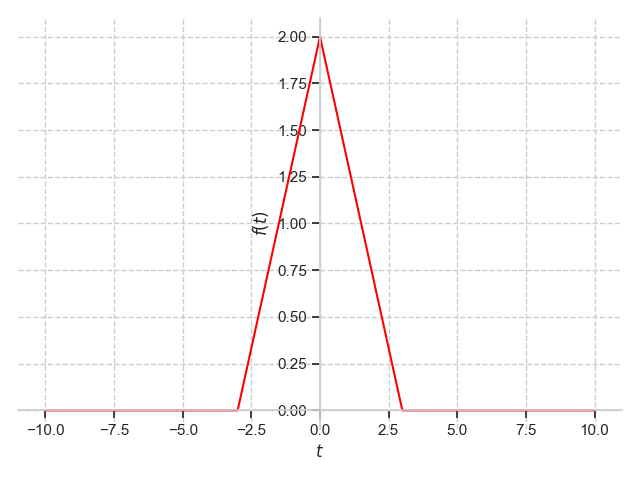
\includegraphics[width=\linewidth]{trif_a=2_b=3.png}
            \caption{$a=2,\,\,b=3$}
            \label{fig:triangf_2}
        \end{subfigure}
        \hfill
        \begin{subfigure}{0.3\textwidth}
            \centering
            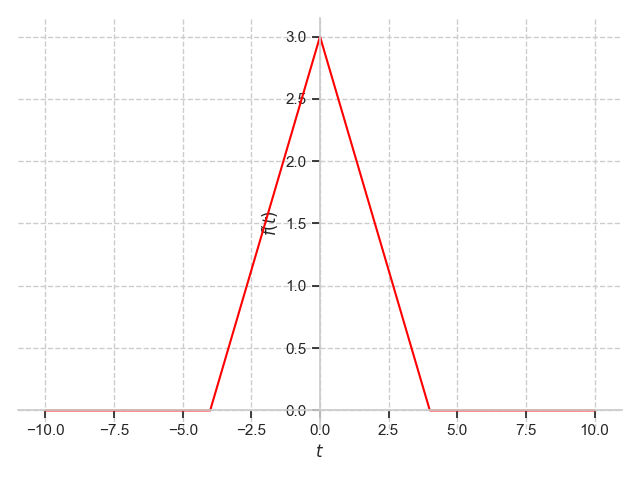
\includegraphics[width=\linewidth]{trif_a=3_b=4.png}
            \caption{$a=3,\,\,b=4$}
            \label{fig:triangf_3}
        \end{subfigure}
        \caption{Треугольные функции при различных значениях $a$ и $b$}
        \label{fig:triangfs}
    \end{figure}
\end{document}